\documentclass{standalone}

\usepackage{lscape}
%Math typesetting packages
\usepackage{amsfonts, amssymb, amsmath, latexsym, amsthm,xparse, bm}
\newcommand\simiid{\stackrel{iid}{\sim}}
\newcommand\simind{\stackrel{ind}{\sim}}
\NewDocumentCommand{\qfrac}{smm}{%
  \dfrac{\IfBooleanT{#1}{\vphantom{\big|}}#2}{\mathstrut #3}%
}

\usepackage{tikz}
\usetikzlibrary{calc,arrows,positioning,shapes,shapes.gates.logic.US,trees, intersections}

\begin{document}

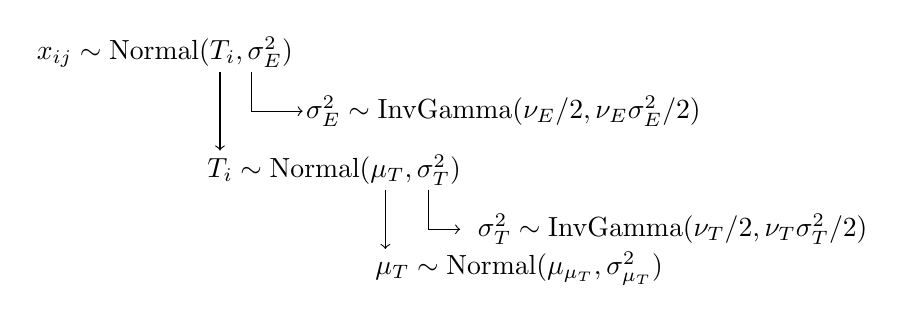
\begin{tikzpicture}
  \node at (0,0) {$x_{ij} \sim \mathrm{Normal}(T_i, \sigma^2_E)$} ;
  	\draw[->] (1.1, -0.25) |- (1.75, -0.75);
  	\node at (4.30, -0.75) {$\sigma^2_E\sim \mathrm{InvGamma}(\nu_E/2, \nu_E\sigma^2_E/2)$};
  	\draw[->] (0.7,-0.25) -- (0.7,-1.25);
  	\node at (2.15, -1.5) {$T_i \sim \mathrm{Normal}(\mu_{T},\sigma^2_{T})$};
  		\draw[->] (3.35, -1.75) |- (3.75, -2.25);
  		\node at (6.45, -2.25) {$\sigma^2_T\sim \mathrm{InvGamma}(\nu_T/2, \nu_T\sigma^2_T/2)$};
  		\draw[->] (2.8, -1.75) -- (2.8, -2.5);
	  	\node at (4.5, -2.75) {$\mu_T \sim \mathrm{Normal}(\mu_{\mu_{T}},\sigma^2_{\mu_T})$};
\end{tikzpicture}

\end{document}